\beginsong{Allzeit Bereit}[mel={Hermann Mettel, 1927}, txt={Johann Heinrich Lützel, 1934}, bo={14}, pfii={1}, pfiii={2}]

\beginverse 
\endverse  
\centering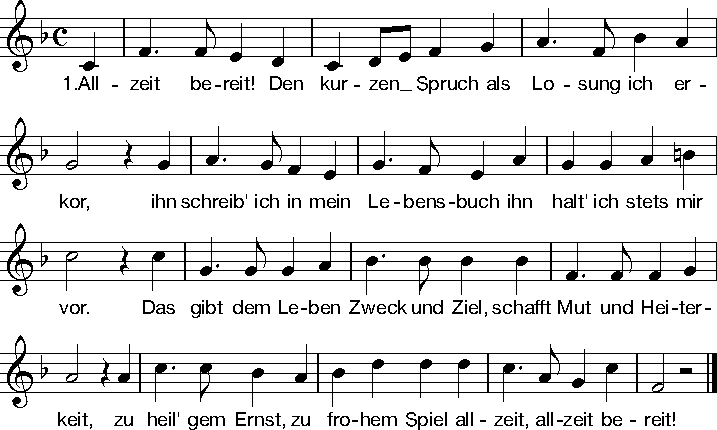
\includegraphics[width=1\textwidth]{Noten/Lied003.pdf}	

\beginverse
Allzeit bereit, dem zu entflieh'n, was mir das Herz befleckt.
Nichts schlechtes soll mich abwärts zieh'n, hoch ist mein Ziel gesteckt.
Gott zum lebend'gen Eigentum sei Leib und Seel' geweiht,
zu seines Namens Ehr' und Ruhm: Allzeit, allzeit bereit!
\endverse

\beginverse
Allzeit bereit, wahr sei der Mund, unwandelbar die Treu'.
Rein sei das Herz, fest sei der Bund, der Wandel ohne Scheu.
So hilf mir Gott, du starker Hort, dass ich kann jederzeit
erfüllen treu das Losungswort: Allzeit, allzeit bereit!
\endverse

\endsong

\beginscripture{}
Bundeslied des VCP, der CPD und anderer christlicher Pfadfinderbünde.
\endscripture
